\documentclass[a4paper, 12pt]{article}
\usepackage{config}

\begin{document}
	\begin{center}
		\begin{huge}
			Resumo dos Comandos
		\end{huge}
	\end{center}

	\begin{itemize}
		\item Lista de comandos a ser tratada
		\begin{itemize}
			\item\ttt{Plot}
			\item\ttt{Plot3D}
			\item\ttt{ContourPlot}
			\item \ttt{ParametricPlot}
			\item\ttt{StreamPlot}
			\item\ttt{VectorPlot}
			\item\ttt{Show}
		\end{itemize}
	\end{itemize}

	\section{Plot}
	Normal recebe uma função que depende de somente uma variável seguida da definição do intervalo de amostragem desejado. Então imagine que se deseja plotar a função do segundo $f(x)=x^{2}$, para fazer isso basta tomar o lado direito da função e utilizar como primeiro parâmetro do \ttt{Plot} como segue.	

	\begin{lstlisting}[language=Mathematica]
	Plot[x^2]
	\end{lstlisting}
	
	Porém, não é adequado parar por aqui, é necessário definir a variação de $x$ em uma dimensão que vai abranger o ``teatro'' escolhido. Dessa maneira, imagine que queiramos plotar essa função de modo a abranger os valores de $x$ que vão de -1 a 1, então aplicamos \ttt{\{x,-1,1\}}. Como consequência, percebe-se que o programa lança valores de $x$ abrangendo o domínio explicitado de modo a conformar a representação gráfica no menor espaço possível de visualização do gráfico para os valores de $x$ propostos
	
	\begin{lstlisting}[language=Mathematica]
	Plot[x^2,{x,-1,1}]
	\end{lstlisting}
	
	Da forma como está, se dermos \ttt{enter} o comando será rodado e vamos obter
	
	\begin{figure}[!h]\label{parabola}
		\centering
		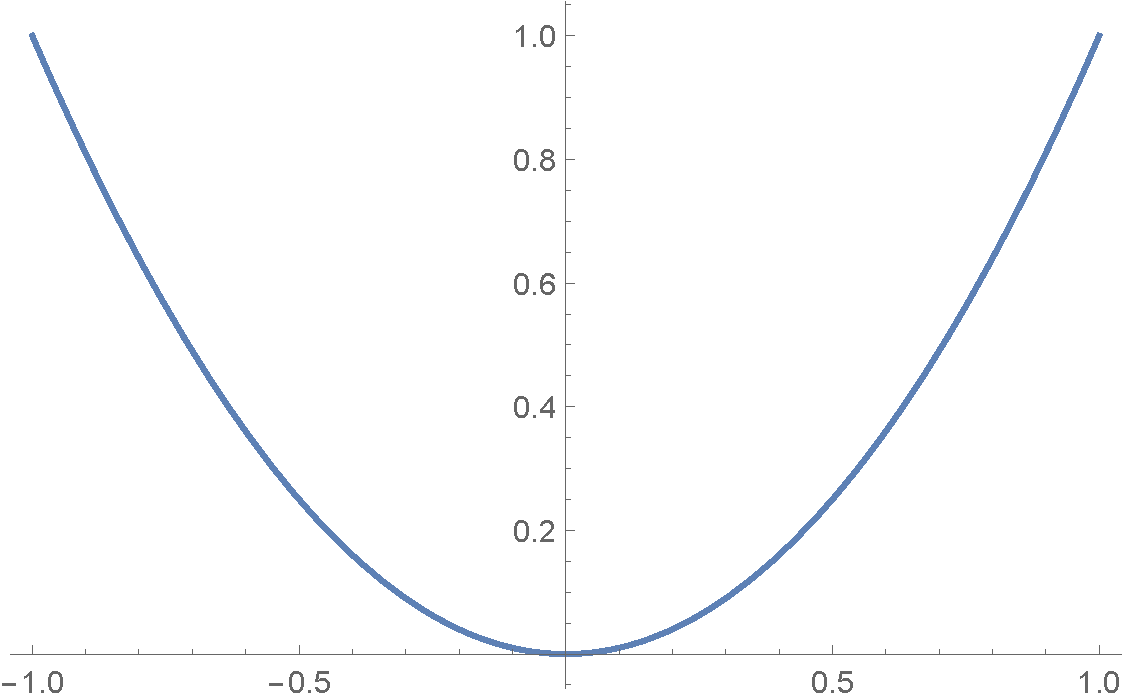
\includegraphics[scale=.5]{images/parabola}
	\end{figure}

	Repare que sendo $x=-1$ ou $x=1$, $f(x)=1$, logo o máximo valor de $f$ mostrado é 1, não precisamos a variação de $y$, até mesmo por que o \ttt{Plot} não aceitaria tal sintaxe. 
	
	\section{Plot3D}
	Podemos interpretar esse comando como expansão do \ttt{Plot}, porém em três dimensões. Sabendo que um ponto no espaço agora depende de $x$ e $y$, consequentemente a função $f(x)$ em duas dimensões passará a ser $f(x,y)$. De forma análoga ao que foi feito para o comando anterior, imagine que queiramos plotar um paraboloide no espaço que obedeça
	
	\begin{equation}
		f(x,y)=x^2+y^2
	\end{equation}
	
	Numa abordagem rápida, podemos imaginar tal superfície como a rotação de uma parábola tal como é visto em \ref{parabola} em torno do eixo $z$ no espaço, então sabendo que dependemos de mais uma variável será preciso acrescentar outro parâmetro ao \ttt{Plot3D} como segue
	
	\begin{lstlisting}[language=Mathematica]
	Plot3D[x^2+y^2,{x,-1,1},{y,-1,1}]
	\end{lstlisting}
	
	\begin{figure}[!h]\label{parabola}
		\centering
		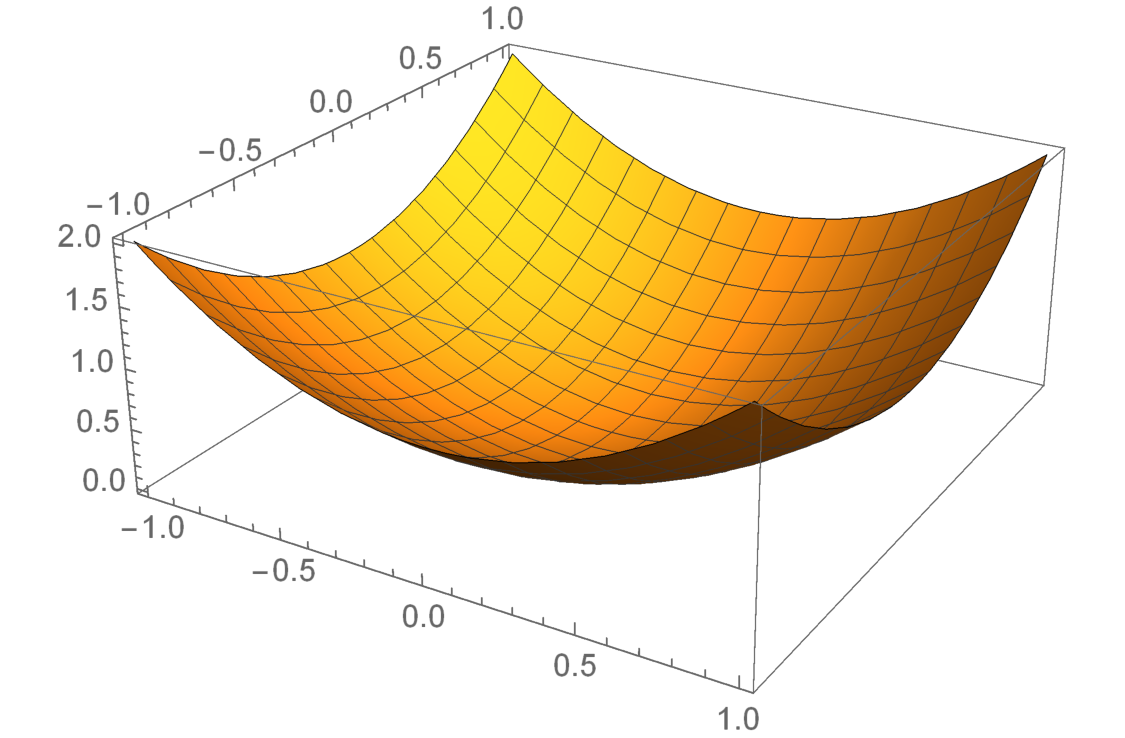
\includegraphics[scale=.6]{images/parabola3d}
	\end{figure}

	Note que se clicarmos com o botão direito do \textit{mouse} e formos na opção \textit{Top View} veremos
	
	\begin{figure}[!h]\label{parabola}
		\centering
		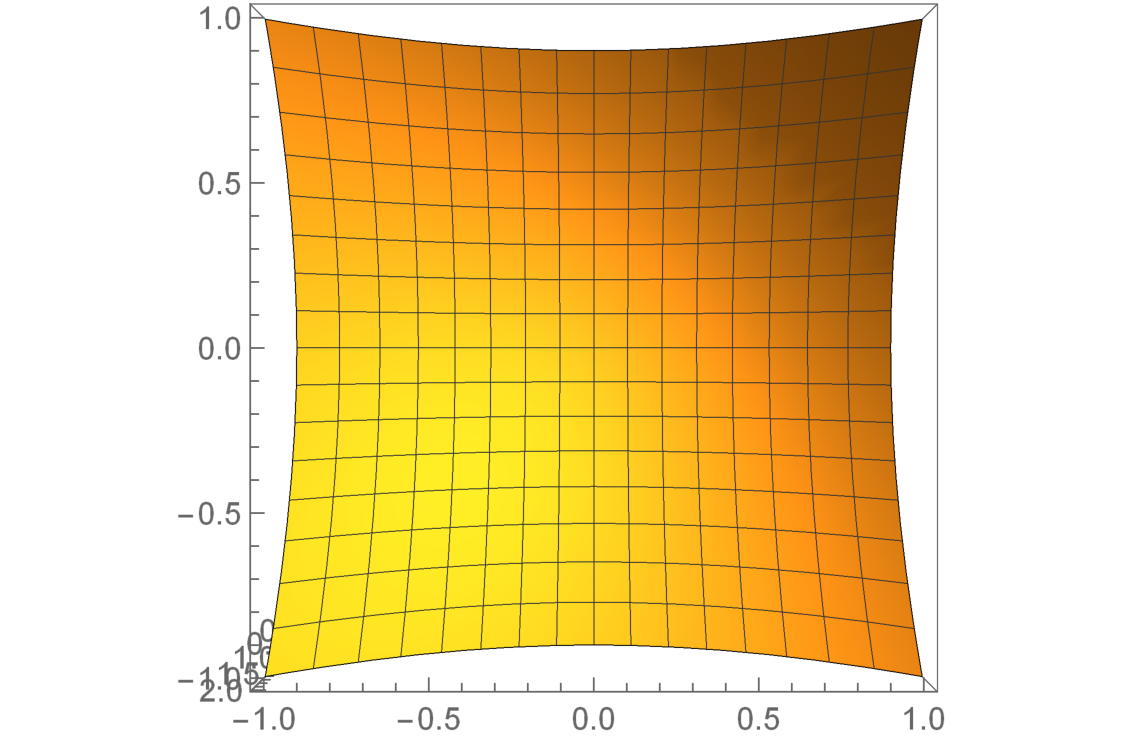
\includegraphics[scale=.55]{images/parabola3dtop}
	\end{figure}
	
	Ou seja, o intervalo de valores escolhido para $x$ e $y$ novamente é notado no domínio presente. Vê-se que a vista superior é um quadrado de lados valendo 2 unidades já que tanto $x$ quanto $y$ variam entre menos -1 e 1.
	
	Partindo para análise em $z$, vamos mudar a opção de \textit{Top View} para \textit{Front View}. Fazendo uma análise visual vemos que a máxima altura da ``caixa'' que comporta o gráfico é de duas unidades. Isso ocorre pois o máximo valor que $f(x,y)$ pode assumir para o domínio escolhido ocorre quando as coordenadas são $(-1,-1)$, $(-1,1)$, $(1,-1)$ ou $(1,1)$ como vemos a seguir
	
	\begin{figure}[!h]\label{parabola}
		\centering
		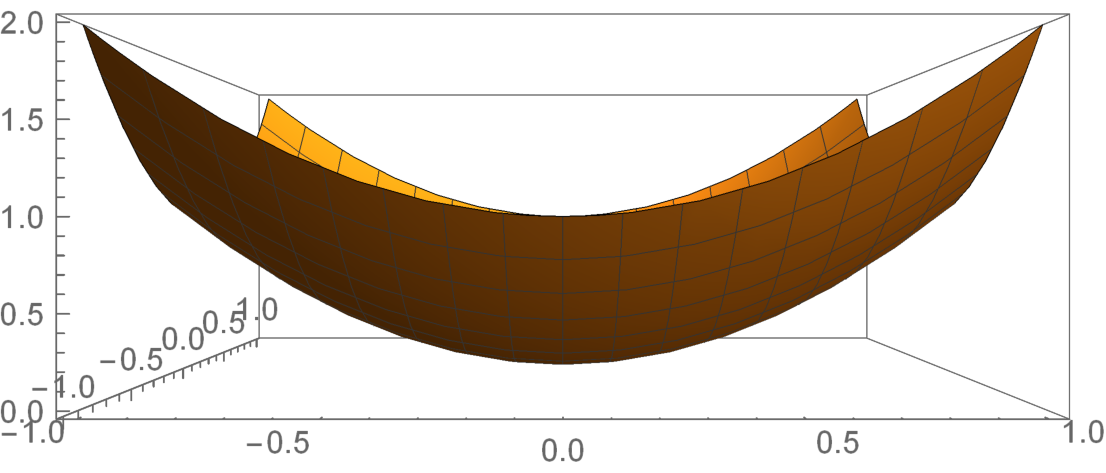
\includegraphics[scale=.55]{images/parabola3dfront}
	\end{figure}

	Sabemos disso devido a simplicidade do gráfico e prevemos que a função é sempre crescente no intervalo dado.
	
	Alguns atributos de estilo podem ser passados para os \ttt{Plot}s de modo a melhorar a visualização ou visando cumprir alguma meta de representação gráfica. Alguns dos comandos a seguir são interessantes de serem entendidos pelo menos no básico.
	
	\vspace{.5cm}
	Para o \ttt{Plot} (Gráficos em 2d no geral) 
	\begin{itemize}
		\item\ttt{AspectRatio}
		\begin{itemize}
			\item Permite editar a proporção entre os eixos do gráfico. Imagine que quiséssemos uma proporção de 1 em $x$ para dois em $y$, teríamos uma razão igual a 0.5 e podemos prever que o gráfico terá maior comprimento em $x$ que em $y$ como vemos a seguir com base nas linhas de comando
		\end{itemize}
	
\begin{lstlisting}[language=Mathematica]
Plot[x^2,{x,-1,1},AspectRatio -> .5]
\end{lstlisting}
		
		\begin{figure}[!h]\label{parabola}
			\centering
			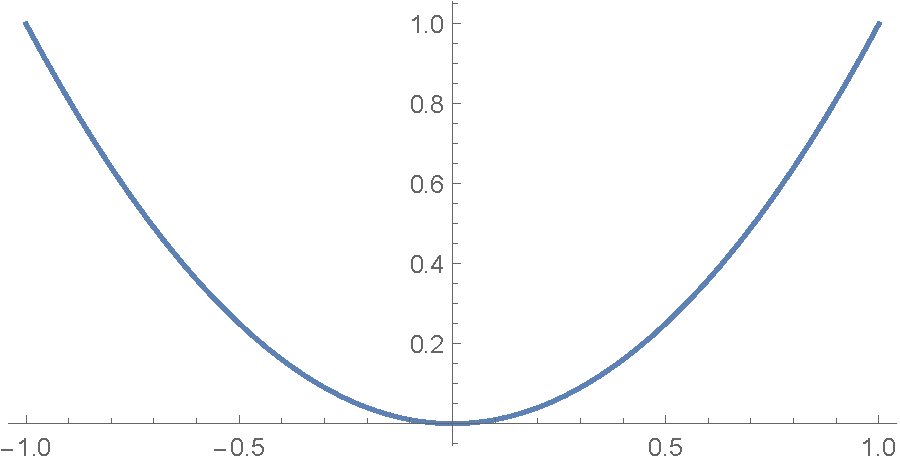
\includegraphics[scale=.55]{images/aspecthalf}
		\end{figure}
		
		Trocando por 2 o valor da propriedade vemos
		
\begin{lstlisting}[language=Mathematica]
Plot[x^2,{x,-1,1},AspectRatio -> 2]
\end{lstlisting}
		
		\newpage 
		\begin{figure}[!h]\label{parabola}
			\centering
			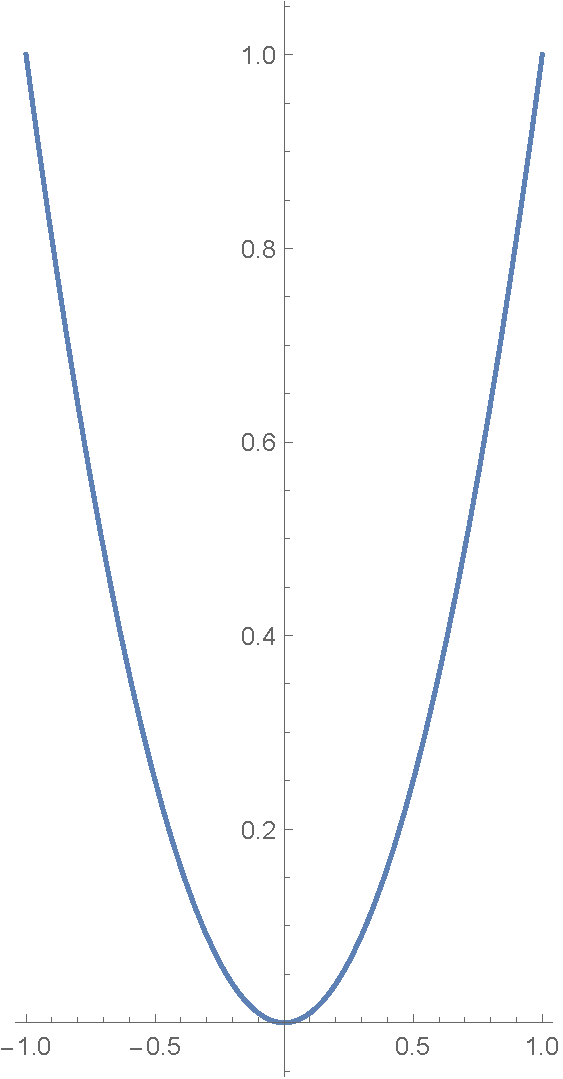
\includegraphics[scale=.55]{images/aspectdouble}
		\end{figure}
	
		\item\ttt{PlotStyle} 
			\begin{itemize}
				\item Um dos atributos mais utilizados, possibilita mudar a cor do gráfico, espessura das linhas, opacidade, entre muitos outros parâmetros. 
				\begin{itemize}
					\item Mudando a cor
					\begin{itemize}
						\item Uma maneira aconselhável é passar diretamente o atributo de cor, como por exemplo \ttt{Magenta}, \ttt{Red}, \ttt{Blue}, \ttt{Cyan} ou utilizar o \ttt{RGBColor} para customizar com maior liberdade como segue
					\end{itemize}
				\end{itemize}
			\end{itemize}
		
\begin{lstlisting}[language=Mathematica]
Plot[x^2,{x,-1,1},AspectRatio -> .5,PlotStyle -> Magenta]
\end{lstlisting}

\begin{figure}[!h]\label{parabola}
	\centering
	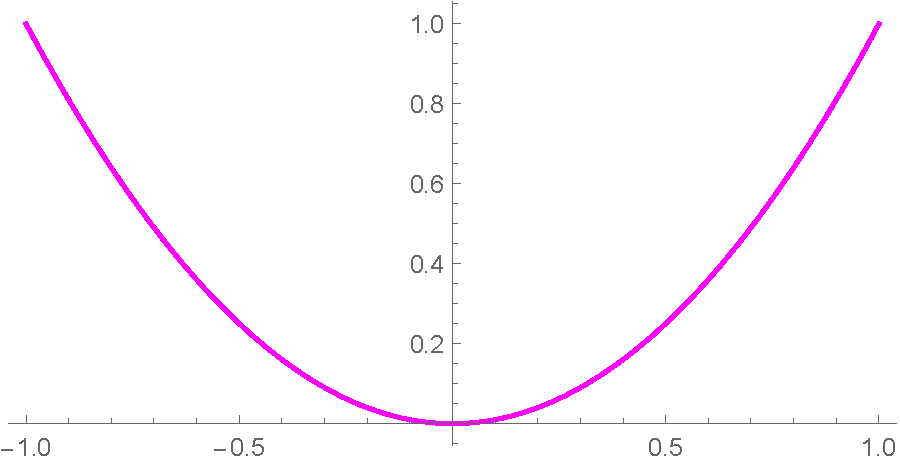
\includegraphics[scale=.55]{images/magenta}
\end{figure}

		\item\ttt{GridLines} 
		\begin{itemize}
			\item Nos permite adicionar uma malha quadriculada ao fundo da plotagem. Esse recurso muitas vezes facilita a associação entre os eixos coordenados e nos permite ter maior precisão quantitativa para aproximações feitas visualmente. Abaixo temos alguns exemplos.
		\end{itemize}


\begin{lstlisting}[language=Mathematica]
Plot[x^2,{x,-1,1},AspectRatio->.5,PlotStyle->Magenta,GridLines->Automatic]
\end{lstlisting}
\begin{figure}[!h]\label{parabola}
	\centering
	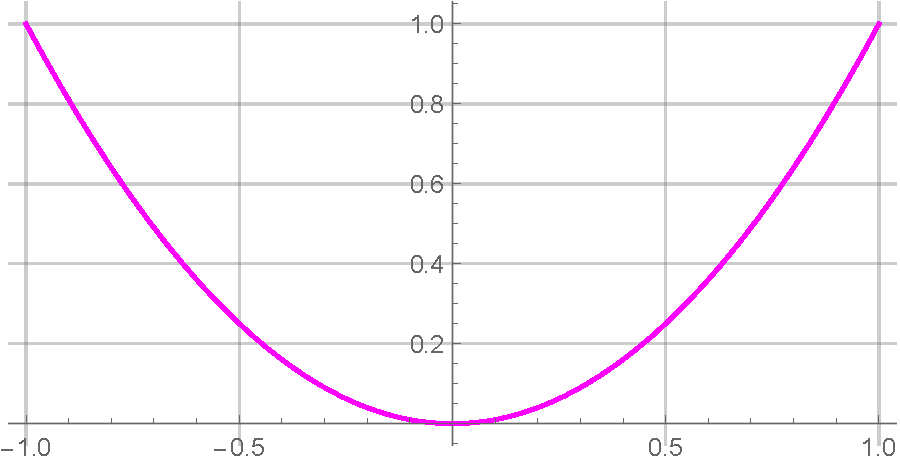
\includegraphics[scale=.55]{images/grid}
\end{figure}
		
		\begin{itemize}
			\item[] Por padrão o \ttt{GridLines} com \ttt{Automatic} renderiza linhas cheias, mas podemos alterálas passando \ttt{GridLinesStyle->\{\{Dashed\},\{Dashed\}\}}. Isso fará com que tanto as linha horizontais quanto as verticais se tornem tracejadas. De forma semelhante usamos o \ttt{Dotted} para deixá-las pontilhadas. O atributo de cor também pode ser passado no interior das chaves como vemos a seguir
		\end{itemize}

\begin{lstlisting}[language=Mathematica]
Plot[x^2,{x,-1,1},AspectRatio->.5,PlotStyle->Magenta,GridLines->Automatic,GridLinesStyle->{{Red, Dotted, Thick},{Gray, Dotted}}}]
\end{lstlisting}
\begin{figure}[!h]\label{parabola}
	\centering
	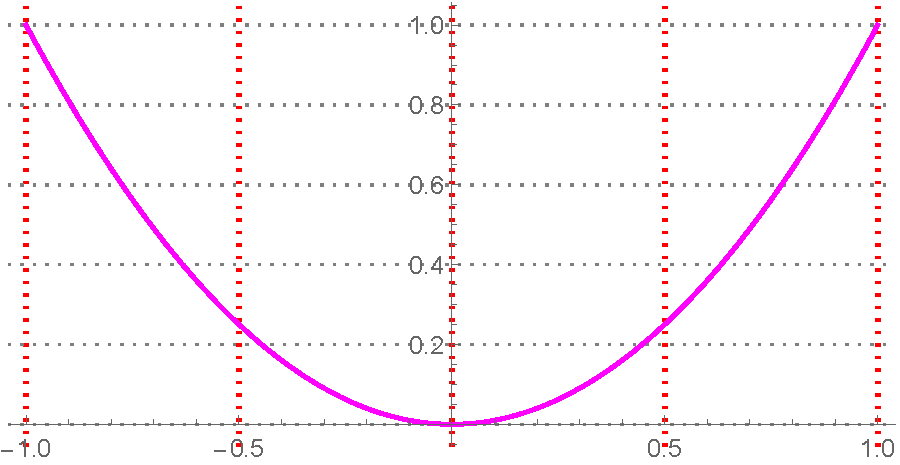
\includegraphics[scale=.85]{images/gridStyle}
\end{figure}

	\begin{itemize}
		\item[] Aumentando-se a proporção do gráfico vê-se que a primeira lista de valores contendo \ttt{Red}, \ttt{Dotted} e \ttt{Thick} tornou as linhas verticais vermelhas, pontilhadas e, como foi passado o \ttt{Thick} houve uma leve aumentada na espessura, somente para melhorar a visualização do leitor.
	\end{itemize}

	\end{itemize}
\end{document}
















